\documentclass{beamer}
\usepackage{lmodern}
\usepackage{anyfontsize}
% \renewcommand{\normalsize}{\fontsize{14}{16}\selectfont}

\usepackage{tikz}

\usepackage{xcolor} % Cargar el paquete para colores

\usetheme{Madrid}
\usecolortheme{default}

\usepackage{xspace}
\newcommand { \onion } {\textit{Onion Routing}\xspace}
\newcommand{\vspc}{\vspace{0.5cm}}

%Information to be included in the title page:
\title[Onion Routing] %optional
{Anonymous Connections and Onion Routing}

\subtitle{
}

\author[] % (optional, for multiple authors)
{
    Seguridad Informática 
}

\institute[LCC - FCEIA] % (optional)
{
    Facultad de Ciencias Exactas, Ingeniería y Agrimensura\\Universidad Nacional de Rosario
}

\date[Seguridad Informática] % (optional)
{Agosto 2025}

\begin{document}

\frame{
    \titlepage
}

\begin{frame}
    \frametitle{Visibilidad en Redes Públicas}
    Cuando uno utiliza una red pública para comunicarse expone:
    \begin{itemize}
        \only<1>{
            \item Quienes hablan.
            \item Desde donde.
            \item Cuan frecuentemente.
            \item De que.
        }
        \only<2>{
            \item \textcolor{violet}{Quienes hablan}.
            \item \textcolor{blue}{Desde donde}.
            \item \textcolor{blue}{Cuan frecuentemente}.
            \item \textcolor{blue}{De que}.
        }
    \end{itemize}

    Esto se debe a muchos de los protocolos subyacentes.

    \pause

    Por distintos motivos podemos querer evitar esta exposición, en particular al análisis del tráfico y a las posibles escuchas.

\end{frame}

\begin{frame}
    \frametitle{\onion}

    Permite la conexiones privadas entre dos puntos\footnote{entre \textit{initiator} y \textit{responder}.}. La red permite evitar saber quien se comunica con quien.

    \vspc

    Los datos cambian su forma a lo largo de la red lo cual contribuye al anonimato en tiempo real en ambas direcciones.

    \vspc

    Tiene un funcionamiento similar al \textit{firewall}. Para las comunicaciones actúa como un paso intermedio en la comunicación pero es una aplicación en si.
\end{frame}

\begin{frame}
    \frametitle{Uso}

    \begin{figure}[h]
        \centering
        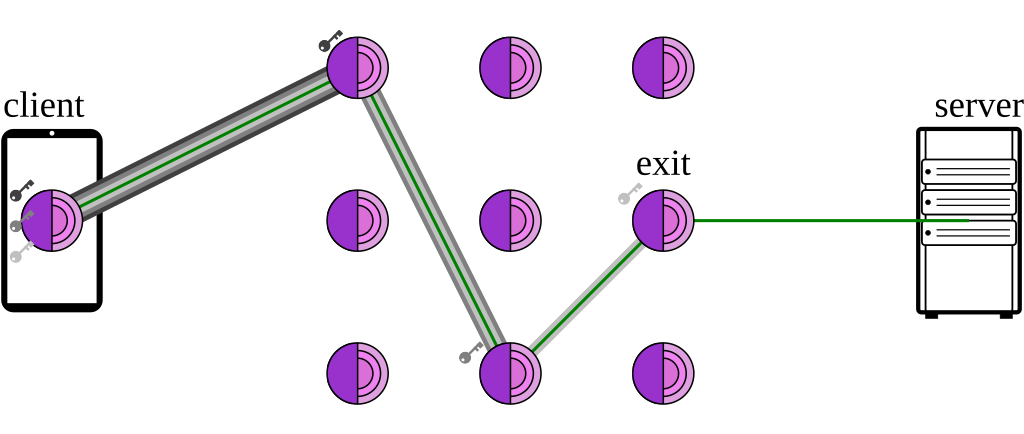
\includegraphics[scale=0.3]{circuitDiagram.png}
        \caption{En este ejemplo se utilizan 3 saltos en lugar de 5}
    \end{figure}
    
\end{frame}

\begin{frame}
    \frametitle{Componentes de la Red}
    \textbf{Proxys}: Adaptación que permite reutilizar aplicaciones existen
    \begin{itemize}
        \item \textbf{Aplicación}: Interfaz entre la aplicación y el siguiente \textit{proxy}. Encargado de aceptar o denegar las conexiones. Estandariza la comunicación, conoce el destino de la comunicación y el protocolo.
        \item \textbf{Onion}: Define la ruta de la conexión anónima. El encargado de construir las cebollas para la comunicación.
    \end{itemize}
    
    
\end{frame}

\begin{frame}
    \frametitle{Componentes de la Red}
    \textbf{Routers}: Nodos intermedios que se encargan de mover la información encriptada. El paso por uno implica quitar una capa de encriptación.
    
    \vspc

    \textbf{Puntos de salida}: Encargado de establecer la conexión con el destinatario fuera de la red. 

\end{frame}

\begin{frame}
    \frametitle{Componentes de la Red}
   
    \textbf{Onions}:
    \begin{columns}
        \column{0.55\textwidth}
            \begin{figure}
            \centering
                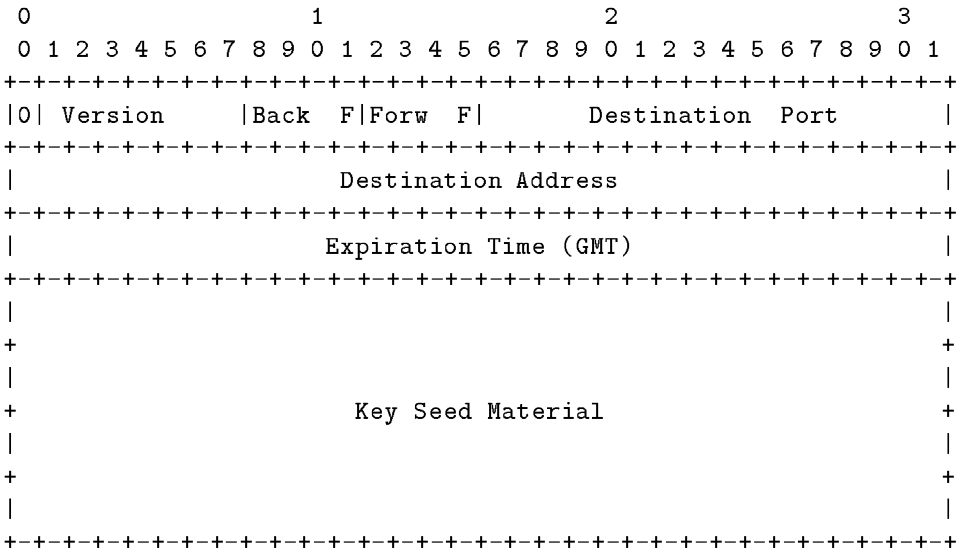
\includegraphics[scale=0.18]{onionConecct.png}
            \end{figure}
        \column{0.4\textwidth}
        
        Es una estructura multi nivel. Cada nivel tiene una forma de encriptar propia. Se utiliza tanto RSA como DES.
    \end{columns}
\end{frame}

\begin{frame}
    \frametitle{Comunicación entre \textit{onion routers}}

    La conexión bidireccional y permanente. Ella multiplexa varias conexione enviando células de tamaño fijo.

    \begin{figure}[h]
        \centering
        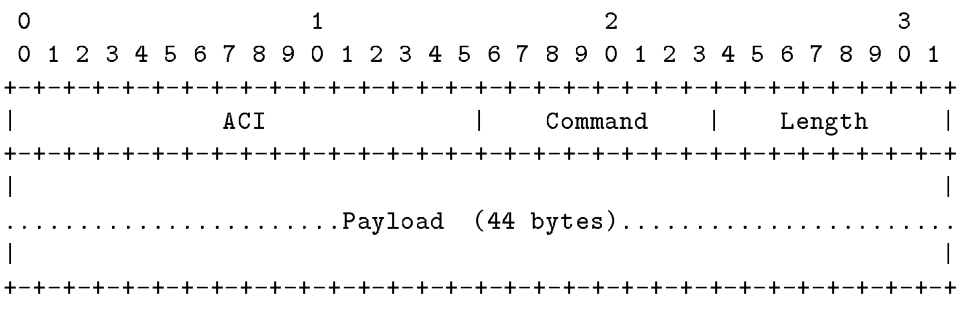
\includegraphics[scale=0.3]{cell.png}
    \end{figure}
\end{frame}

\begin{frame}
    \frametitle{Prueba Empírica}

    Dentro de una misma computadora se configuró una red.

    \vspc

    \begin{itemize}
        \item Contaba con 5 nodos.
        \item La sobrecarga viene de la criptografía.
        \item No se puede medir nociones de latencia.
    \end{itemize}
\end{frame}

\begin{frame}
    \frametitle{Red de Prueba}

    Se montó una red de prueba con 13 nodos abierta al público

    \vspc

    \begin{figure}[h]
        \centering
        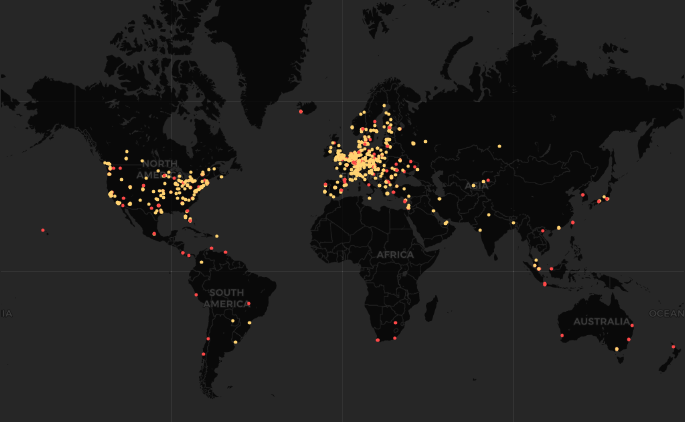
\includegraphics[scale=0.3]{tpo_tor.png}
        \caption{La red TOR hoy cuenta con más de 7 mil routers.\footnote{https://metrics.torproject.org/networksize.html}}
    \end{figure}

    % La red TOR hoy cuenta con más de 7 mil routers.\footnote{https://metrics.torproject.org/networksize.html}
\end{frame}

\begin{frame}
    \frametitle{Ataques Conocidos}
    
    El principal objetivo de un atacante es identificar quienes se están comunicando y desde donde lo hacen.\\

    \vspc

    La red es puede sufrir dos tipos de ataques:
    \begin{itemize}
        \item Pasivos: no hay modificaciones
        \item Activos: se manipulan paquetes o la red misma.
    \end{itemize}

\end{frame}

\begin{frame}
    \frametitle{Ataques Conocidos}
    \textbf{Ataque de marcado\footnote{Marker attack}}: Interceptando distintas marcas distintivas propias de los mensajes, se buscaría descubrir (o deducir) cuál es el próximo paso al que va el mensaje.\\
    
    \vspc

    \textbf{Ataque por tiempo\footnote{Timing attack}}: Utilizando el tiempo de los mensajes.\\

    \vspc

    Los dos ataques requieren tener al menos 2 routers comprometidos. Su mitigación es mantener la red uniformemente ocupada.

\end{frame}

\begin{frame}
    \frametitle{Ataques Conocidos}
    \textbf{Ataque compartiendo cantidad de paquetes vistos}: Nodos comprometidos podrían compartir entre ellos la cantidad de paquetes de una sesión.\\
    
    \vspc

    \textbf{Ataque por modificación del tráfico}: Generar perturbaciones en una sesión para que las cambios de frecuencia de las células.\\

\end{frame}

\begin{frame}
    \frametitle{Vulnerabilidades de la implementación}

    \begin{itemize}
        \item Manejo de colas. (Causando demoras).
        \item Problemas con la generación de números aleatorios (para el padding).
        \item Caídas de nodos en la red.
        \item Errores en la implementación de los métodos criptográficos.
    \end{itemize}

\end{frame}

\begin{frame}
    \frametitle{Uso de la red}
    \begin{itemize}
        \item Redes virtuales privadas. 
        \item Chats anónimos.
        % \item Monedas anónimas.
        \item Acceso remoto.
        \item Búsqueda web.
        \item Servicio de email.
    \end{itemize}
\end{frame}

\begin{frame}
    \frametitle{Conclusiones}
    \begin{itemize}
        \item Se puede separar el anonimato de la conexión de la comunicación.
        \item Se puede aplicar a muchos de los protocolos existentes.
        \item El protocolo actúa como una aplicación propia interponiéndose en las comunicaciones.
    \end{itemize}
\end{frame}


\end{document}